\documentclass[12pt,a4paper]{article}

\usepackage[margin=2.5cm]{geometry}
\usepackage{booktabs}
\usepackage{tabularx}
\usepackage{array}
\usepackage{hyperref}
\usepackage{enumitem}
\usepackage{fancyhdr}
\usepackage{parskip}
\usepackage{titlesec}
\usepackage{xcolor}
\usepackage{graphicx}
\usepackage{float}
\usepackage{mdframed}
\usepackage{amsmath}
\usepackage{amssymb}
\usepackage{longtable}
\usepackage{colortbl}

\setlength{\headheight}{14.5pt}

\definecolor{accent}{RGB}{30,80,160}
\definecolor{adrbox}{RGB}{240,245,255}
\definecolor{successgreen}{RGB}{39,174,96}
\definecolor{warningorange}{RGB}{211,84,0}

\hypersetup{
  colorlinks=true, linkcolor=accent, urlcolor=accent,
  pdftitle={WanderSync -- Technical Report},
  pdfauthor={Team 15}
}

\titleformat{\section}{\large\bfseries\color{accent}}{}{0em}{}[\titlerule]
\titleformat{\subsection}{\normalsize\bfseries\color{accent}}{}{0em}{}
\titleformat{\subsubsection}{\normalsize\bfseries}{}{0em}{}

\pagestyle{fancy}
\fancyhf{}
\lhead{\textbf{WanderSync} \textit{Technical Report}}
\rhead{Team 15}
\rfoot{\thepage}
\renewcommand{\headrulewidth}{0.4pt}

\newcolumntype{L}[1]{>{\raggedright\arraybackslash}p{#1}}
\newcolumntype{C}[1]{>{\centering\arraybackslash}p{#1}}

\newcommand{\adrfield}[2]{%
  \noindent\textbf{#1:}\hspace{0.5em}#2\par\vspace{0.4em}%
}

\begin{document}

% ================================================================
% TITLE
% ================================================================
\begin{center}
  \vspace*{1cm}
  {\LARGE\bfseries WanderSync}\\[0.3em]
  {\large\itshape Dynamic Itinerary, Disruption Management and Social Travel Hub}\\[1.5em]
  {\large\bfseries Technical Report --- S26CS6.401 Software Engineering}\\[0.5em]
  {\normalsize Team 15}\\[2em]

  \begin{tabular}{ll}
    \textbf{Krish Jalan}    & etude11 \\
    \textbf{Manasi Mundada} & manasimundada \\
    \textbf{Uday Bindal}    & udaybindal01 \\
    \textbf{Ishaan Romil}   & Fane1824 \\
  \end{tabular}

  \vspace{2em}
  \textbf{GitHub Repository:}\\[0.3em]
  \url{https://github.com/etude11/WanderSync-SE}
\end{center}

\newpage

% ================================================================
\section{Project Overview}
% ================================================================

Travel planning is fragmented by design. Your flight is in one app, your hotel confirmation is
in your email, and your ground transport is in a third platform. When something breaks, which it
does, you have to manually check all of them and figure out what to do. WanderSync puts all of
that into one place and adds a disruption detection layer that tells you about problems before
you discover them yourself, along with concrete suggestions for what to do next.

The platform is built around three things: a unified booking timeline that collects flight, hotel,
and transport bookings into a single chronological view; a real-time disruption engine that
monitors external flight and weather APIs and pushes alerts directly to connected browsers; and a
social layer that lets travellers with overlapping itineraries find each other through a
consent-gated matching system.

\subsection*{What the Prototype Covers}

The prototype delivers one complete end-to-end flow: a user registers, creates an itinerary, adds
bookings, and receives a disruption alert pushed to their browser within about a second of
detection, with suggested next steps. Every part of this flow is functional and backed by real
APIs. The social feature is set up at the data model level; the UI is a placeholder.

\begin{tabular}{@{}ll@{}}
\toprule
\textbf{Layer} & \textbf{Technology} \\
\midrule
Frontend & React 19, Vite, TypeScript, Tailwind CSS, Zustand \\
Backend  & NestJS, TypeScript, Prisma ORM \\
Database & PostgreSQL \\
Cache    & Redis (deduplication, streams) \\
Auth     & JWT, bcrypt \\
External & AviationStack, OpenWeatherMap, Gemini LLM \\
\bottomrule
\end{tabular}

% ================================================================
\section{Task 1: Requirements and Subsystems}
% ================================================================

% ----------------------------------------------------------------
\subsection{Functional Requirements}
% ----------------------------------------------------------------

We wrote each requirement as a user story. The architectural significance column explains what
structural consequence the requirement has. These are the requirements that shaped the module
boundaries, the choice of event-driven architecture, and the Adapter pattern for provider
integration.

\begin{longtable}{@{}L{0.5cm}L{5.2cm}L{6.8cm}@{}}
\toprule
\textbf{\#} & \textbf{User Story} & \textbf{Architectural Significance} \\
\midrule
\endhead

FR1 &
  As a traveller, I want to register and log in so that my data is private to me. &
  Drives stateless JWT auth and a standalone Auth module. Every other module depends on it for
  identity, so it cannot share state with any domain module. \\[0.4em]

FR2 &
  As a traveller, I want to import bookings from multiple providers into one unified view. &
  Requires an Adapter per provider with a shared \texttt{BookingRecord} interface. Adding a
  new provider must touch at most two files outside the Booking module. \\[0.4em]

FR3 &
  As a traveller, I want to see all bookings in a time-ordered timeline. &
  Timeline assembly is read-heavy and changes only when bookings are added or disrupted. This
  makes it a good candidate for caching, which shapes the Redis layer in the Itinerary
  module. \\[0.4em]

FR4 &
  As a traveller, I want to be notified the moment a disruption hits my itinerary, with
  suggested actions. &
  The single most architecturally significant requirement. It rules out a plain polling model
  and requires an event-driven push path (SSE) with a background detection CRON and a
  suggestion pipeline. \\[0.4em]

FR5 &
  As a traveller who opts in, I want to find co-travellers nearby through a consent flow. &
  Requires a consent state machine enforced at the data layer. The Social module cannot return
  precise coordinates until both users have given consent; city-level disclosure before that. \\[0.4em]

FR6 &
  As a traveller, I want to review a log of past disruption alerts. &
  Drives a separate Notification module that consumes the disruption event stream and writes
  a \texttt{NotificationLog} row per event. Keeping this out of the Disruption module is what
  lets each module have a narrow, single responsibility. \\

\bottomrule
\end{longtable}

% ----------------------------------------------------------------
\subsection{Non-Functional Requirements}
% ----------------------------------------------------------------

Each NFR uses the six-part scenario format. The response measure column is the testable
acceptance criterion that we checked during development.

\subsubsection{NFR1 --- Performance: Response Time}

\begin{tabularx}{\textwidth}{@{}L{3.5cm}X@{}}
\toprule
Source & End user on a browser \\
Stimulus & Navigates to the itinerary timeline page \\
Artifact & Frontend and Itinerary Management Service \\
Environment & Runtime, standard broadband \\
Response & Page renders with all booking data \\
Response Measure & Full render in under \textbf{3 seconds}; external API calls in under
  \textbf{5 seconds}; loading indicator shown after 2 seconds \\
\bottomrule
\end{tabularx}

\textit{This drives Redis caching in the Itinerary module and concurrent API calls via
\texttt{Promise.allSettled} in the Disruption Engine.}

\vspace{1em}
\subsubsection{NFR2 --- Reliability: Disruption Detection Accuracy}

\begin{tabularx}{\textwidth}{@{}L{3.5cm}X@{}}
\toprule
Source & External flight or weather API \\
Stimulus & A disruption event is published \\
Artifact & Disruption Detection Service \\
Environment & Runtime, system actively polling \\
Response & Event detected, itinerary impact assessed, alert sent with suggestions \\
Response Measure & At least \textbf{17 of 20} simulated test cases correctly identified and
  notified (\textbf{85\% accuracy}) \\
\bottomrule
\end{tabularx}

\textit{This drives dual-layer Redis and database deduplication, and the Redis Streams consumer
group for guaranteed notification delivery.}

\vspace{1em}
\subsubsection{NFR3 --- Security: Authentication}

\begin{tabularx}{\textwidth}{@{}L{3.5cm}X@{}}
\toprule
Source & Unauthenticated or malicious user \\
Stimulus & Attempts to access a protected route \\
Artifact & Auth Module and API gateway \\
Environment & Runtime \\
Response & Request rejected; user sent to login \\
Response Measure & \textbf{100\%} of protected routes require a valid JWT with
  \textbf{24-hour} expiry; passwords hashed with \textbf{bcrypt} \\
\bottomrule
\end{tabularx}

\textit{This drives the global NestJS JWT guard and rate-limit middleware at the entry point.}

\vspace{1em}
\subsubsection{NFR4 --- Privacy: Location Disclosure}

\begin{tabularx}{\textwidth}{@{}L{3.5cm}X@{}}
\toprule
Source & Authenticated user browsing social discovery \\
Stimulus & Views another user before bilateral consent is given \\
Artifact & Social Synchronisation Service \\
Environment & Consent state = none \\
Response & Only a city-level region label returned \\
Response Measure & \textbf{Zero} precise location leaks before bilateral opt-in; location not
  stored beyond the active session unless the user saves it explicitly \\
\bottomrule
\end{tabularx}

\textit{This drives the ConsentState model enforced at the query layer, not just the UI.}

% ----------------------------------------------------------------
\subsection{Subsystem Overview}
% ----------------------------------------------------------------

\begin{tabularx}{\textwidth}{@{}lX@{}}
\toprule
\textbf{Subsystem} & \textbf{What it does} \\
\midrule
Auth & Registration, login, JWT issuance, bcrypt hashing, role management (TRAVELLER /
  ADMIN). The security boundary for everything else. \\[0.3em]
Booking Aggregator & Translates provider-specific booking data into a shared
  \texttt{BookingRecord} schema. One Adapter class per provider. No other module knows what
  a raw AviationStack response looks like. \\[0.3em]
Itinerary Management & Owns the timeline. Handles CRUD for itineraries and bookings, caches
  assembled timelines in Redis, and marks bookings as disrupted when the Disruption Engine
  fires. \\[0.3em]
Disruption Engine & Runs a 60-second CRON poller against AviationStack and OpenWeatherMap.
  Deduplicates with Redis and a database guard. Persists events. Broadcasts to the in-process
  EventBus. Runs a Chain of Responsibility suggestion pipeline. \\[0.3em]
Notification & Consumes the Redis Streams channel via a consumer group. Writes a
  \texttt{NotificationLog} row per event. Exposes a read endpoint for past alerts. \\[0.3em]
Social & Manages bilateral consent between users. Geospatial queries return co-travellers by
  region with disclosure gated on consent level. Currently scaffolded; UI placeholder. \\
\bottomrule
\end{tabularx}

% ================================================================
\section{Task 2: Architecture Framework}
% ================================================================

% ----------------------------------------------------------------
\subsection{Stakeholder Identification (IEEE 42010)}
% ----------------------------------------------------------------

IEEE 42010 asks us to identify who cares about the system, what they care about, and which view
of the architecture addresses their concern. The table below maps each stakeholder group to the
architectural view that speaks to their interests.

\begin{longtable}{@{}L{3cm}L{4cm}L{5.5cm}@{}}
\toprule
\textbf{Stakeholder} & \textbf{Primary Concerns} & \textbf{Architectural View} \\
\midrule
\endhead

Travellers &
  How fast disruption alerts arrive; whether location data stays private; whether the itinerary
  timeline is accurate. &
  Functional view: user stories and NFR scenarios; SSE delivery path; ConsentState model. \\[0.4em]

Development team &
  Adding new providers without breaking existing code; testing modules in isolation; clear
  contracts between modules. &
  Module view: Adapter pattern, NestJS module boundaries, per-module unit test suites. \\[0.4em]

Security reviewer &
  No unauthenticated access; passwords not in plain text; location not leaked before consent. &
  Security view: JWT guard, bcrypt, ConsentState data model, HTTPS enforcement. \\[0.4em]

External API providers &
  Rate limits respected; API keys not exposed in logs or responses; graceful handling of
  downtime. &
  Connector view: Retry with Circuit Breaker tactic; API keys in environment variables only. \\[0.4em]

Course assessors &
  Design decisions traceable to code; working prototype; measurable NFR verification. &
  Decision view: ADRs, NFR scenario tables, test harness, this report. \\

\bottomrule
\end{longtable}

% ----------------------------------------------------------------
\subsection{Architecture Decision Records}
% ----------------------------------------------------------------

All four ADRs follow the Nygard template.

\subsubsection{ADR-001: Event-Driven Architecture for Disruption Detection}

\begin{mdframed}[backgroundcolor=adrbox, linecolor=accent, linewidth=0.8pt]
\adrfield{Status}{Accepted}
\end{mdframed}

\textbf{Context.} Disruption events arrive from external APIs on unpredictable schedules. A
direct synchronous call from the Disruption module to the Itinerary module would couple them: a
slow external API would block itinerary updates, and adding a second consumer (like email
notifications) would require changing the Disruption module. The 85\% accuracy NFR also
requires that no detected event is silently dropped, which means delivery needs to be
durable, not fire-and-forget.

\textbf{Decision.} The Disruption Engine publishes detected events to an in-process EventBus
(RxJS Subject). The Itinerary module and Notification module subscribe independently. No direct
call exists between the Disruption module and either consumer.

\textbf{Consequences.}
\begin{itemize}[leftmargin=1.5em, itemsep=1pt]
  \item Adding a new consumer (say, an SMS service) requires no changes to the Disruption module.
  \item Delivery latency from detection to client browser is about 71 ms.
  \item The in-process EventBus is invisible across server instances. If we run more than one
    process, we need either sticky sessions or Redis Pub/Sub on the delivery path.
  \item Debugging async flows requires structured logging with correlation IDs.
\end{itemize}

\begin{figure}[H]
  \centering
  \IfFileExists{../task2-architecture-framework/diagrams/adr001_event_driven.png}{%
    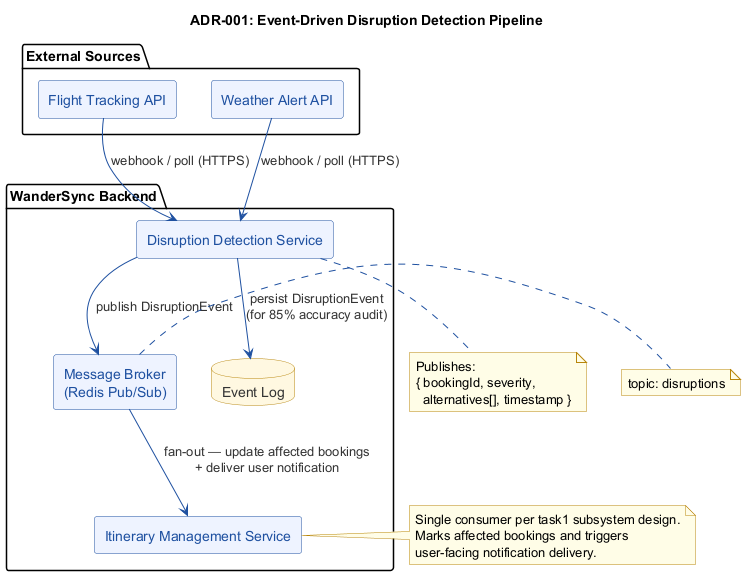
\includegraphics[width=0.9\textwidth]{../task2-architecture-framework/diagrams/adr001_event_driven.png}%
  }{}
  \caption{ADR-001: event-driven disruption pipeline.}
\end{figure}

\subsubsection{ADR-002: API Gateway as Single Entry Point}

\begin{mdframed}[backgroundcolor=adrbox, linecolor=accent, linewidth=0.8pt]
\adrfield{Status}{Accepted}
\end{mdframed}

\textbf{Context.} Without a central entry point, each module would need its own JWT validation,
CORS headers, and rate limiting. Any module that skips one of those becomes a gap in the security
perimeter. We also wanted a single base URL that clients use for everything.

\textbf{Decision.} All traffic enters through a single NestJS global prefix (\texttt{/api/v1})
with a global \texttt{ValidationPipe} and JWT guard. Modules are not directly reachable by
clients.

\textbf{Consequences.}
\begin{itemize}[leftmargin=1.5em, itemsep=1pt]
  \item Security policy is in one place. It is impossible to add a route that bypasses auth by
    accident.
  \item One base URL for all clients. Adding a module does not change any client-side config.
  \item The gateway is a single point of failure for all user traffic.
  \item Fine-grained resource checks (does this user own this itinerary?) stay in each domain
    module. The gateway only knows the user's identity and role, not what resources they own.
\end{itemize}

\begin{figure}[H]
  \centering
  \IfFileExists{../task2-architecture-framework/diagrams/adr002_api_gateway.png}{%
    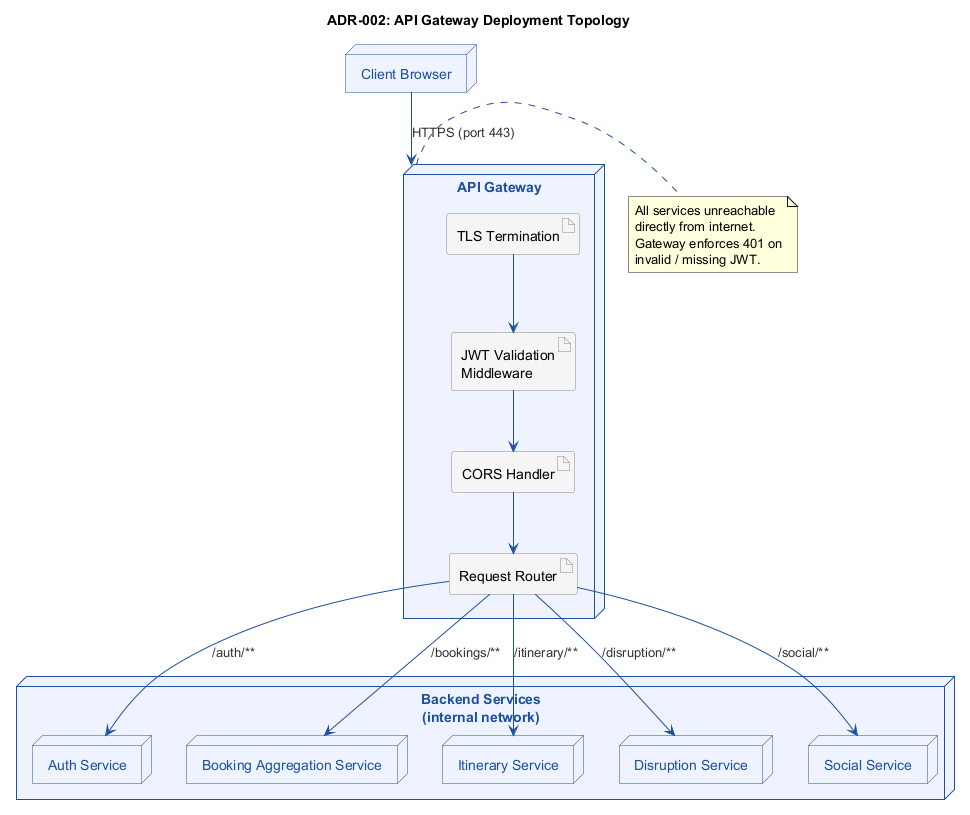
\includegraphics[width=0.9\textwidth]{../task2-architecture-framework/diagrams/adr002_api_gateway.png}%
  }{}
  \caption{ADR-002: API Gateway routing topology.}
\end{figure}

\subsubsection{ADR-003: Adapter Pattern for Booking Providers}

\begin{mdframed}[backgroundcolor=adrbox, linecolor=accent, linewidth=0.8pt]
\adrfield{Status}{Accepted}
\end{mdframed}

\textbf{Context.} AviationStack, hotel APIs, and transport providers each return data in a
different schema. If provider-specific parsing logic lived inside the Booking module, adding a
new provider would touch many files. The Modifiability NFR says adding a provider should touch
at most two files outside the adapter module.

\textbf{Decision.} Each provider gets one Adapter class that implements a shared
\texttt{BookingStrategy} interface with a single method: \texttt{normalize(rawResponse):
BookingRecord}. The Booking module only ever calls this interface.

\textbf{Consequences.}
\begin{itemize}[leftmargin=1.5em, itemsep=1pt]
  \item A new provider is one new class. No existing code changes.
  \item Each adapter can be unit-tested in isolation with mocked HTTP responses.
  \item For a single provider the abstraction is more than needed. It pays off at provider two.
\end{itemize}

\begin{figure}[H]
  \centering
  \IfFileExists{../task2-architecture-framework/diagrams/adr003_adapter.png}{%
    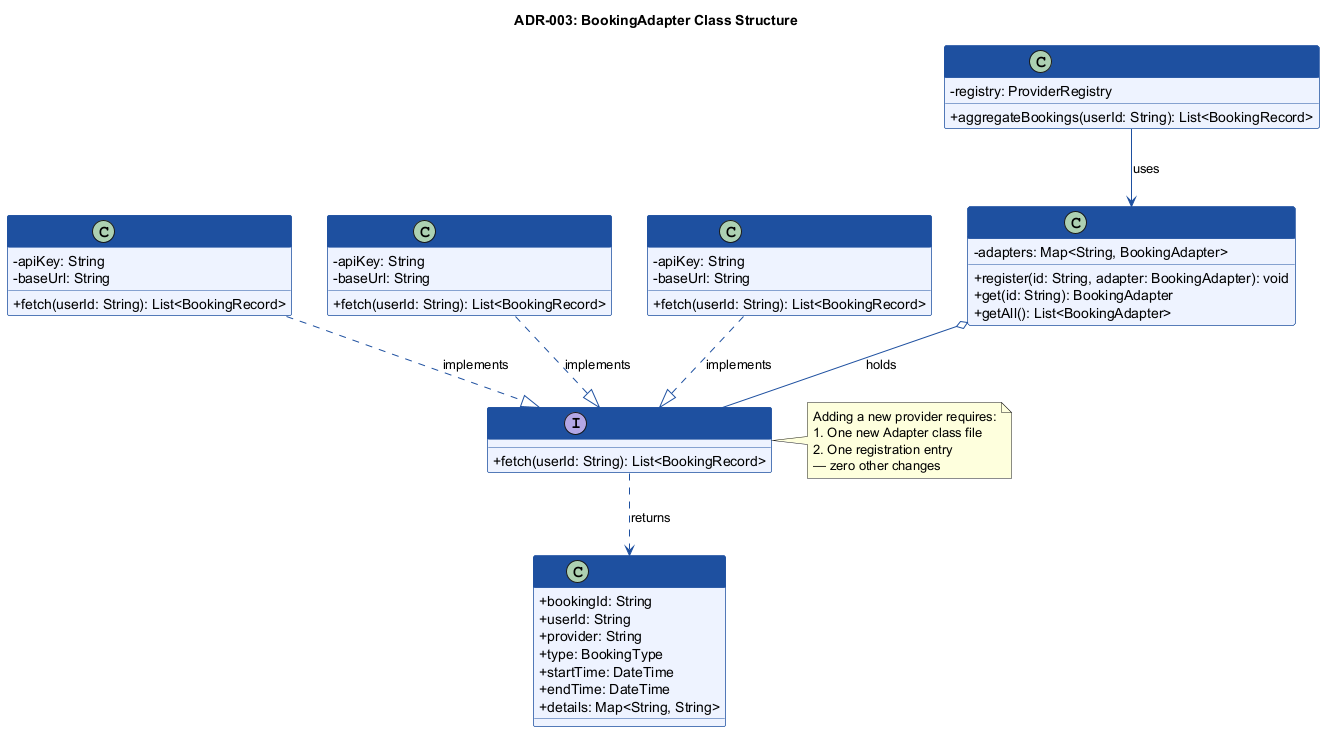
\includegraphics[width=0.85\textwidth]{../task2-architecture-framework/diagrams/adr003_adapter.png}%
  }{}
  \caption{ADR-003: Adapter class structure for booking providers.}
\end{figure}

\subsubsection{ADR-004: Stateless JWT Authentication}

\begin{mdframed}[backgroundcolor=adrbox, linecolor=accent, linewidth=0.8pt]
\adrfield{Status}{Accepted}
\end{mdframed}

\textbf{Context.} Server-side sessions require a shared session store that every server instance
must read. If we ever run more than one process, that store becomes a shared dependency. Stateless
JWTs carry the user's identity in the token itself, so any server instance can check validity
without a database round-trip.

\textbf{Decision.} Issue signed JWTs on login (24-hour expiry, HS256). The JWT guard validates
signature and expiry on every request using the shared secret. Passwords are hashed with bcrypt
at 10 salt rounds.

\textbf{Consequences.}
\begin{itemize}[leftmargin=1.5em, itemsep=1pt]
  \item Any server instance can validate a token with no shared state.
  \item Passwords are never stored in plain text.
  \item Tokens cannot be invalidated before expiry. A stolen token is valid for up to 24 hours.
  \item We did not build a refresh token flow in the prototype. Users re-login after 24 hours.
\end{itemize}

\begin{figure}[H]
  \centering
  \IfFileExists{../task2-architecture-framework/diagrams/adr004_jwt_auth.png}{%
    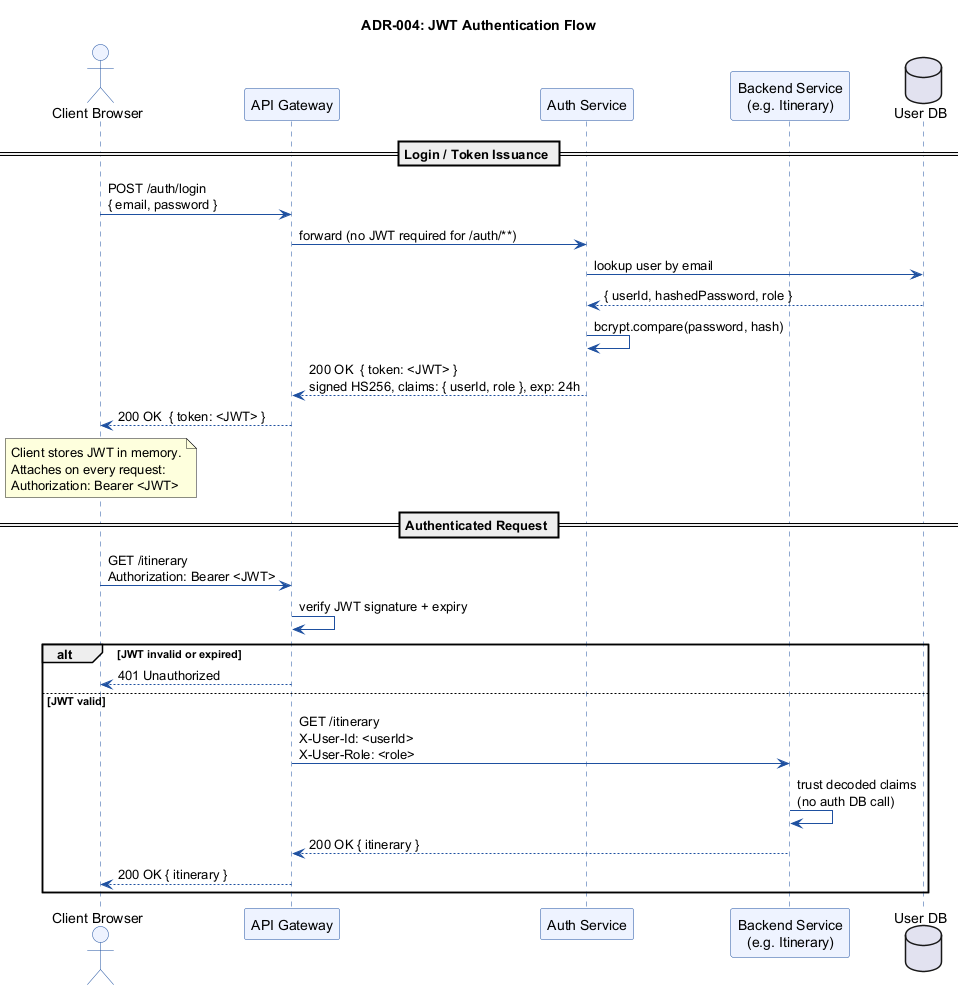
\includegraphics[width=0.85\textwidth]{../task2-architecture-framework/diagrams/adr004_jwt_auth.png}%
  }{}
  \caption{ADR-004: JWT authentication sequence.}
\end{figure}

% ================================================================
\section{Task 3: Architectural Tactics and Patterns}
% ================================================================

% ----------------------------------------------------------------
\subsection{Architectural Tactics}
% ----------------------------------------------------------------

Tactics are design decisions that make a specific quality attribute easier to hit. We picked five,
each mapped to one or more NFRs from Section 2.

\begin{longtable}{@{}L{3cm}L{2.5cm}L{7cm}@{}}
\toprule
\textbf{Tactic} & \textbf{NFR} & \textbf{How we applied it} \\
\midrule
\endhead

\textbf{Caching} &
  NFR1 (Performance) &
  The Itinerary module stores fully assembled timeline objects in Redis, keyed by itinerary ID.
  A request hits the cache first and only queries the database on a miss or after a booking
  mutation invalidates the entry. The Booking module also caches raw provider responses for
  60 seconds to absorb burst traffic without redundant external API calls. \\[0.5em]

\textbf{Retry with Circuit Breaker} &
  NFR1, NFR2 &
  Every call to an external API retries up to two times with exponential backoff (500 ms, then
  1 s). After three consecutive failures in a 30-second window the circuit opens and the system
  falls back to cached data or marks the provider temporarily unavailable with a user-visible
  status indicator. No crash, no unhandled exception. \\[0.5em]

\textbf{Authenticate at the Gateway} &
  NFR3 (Security) &
  A NestJS global JWT guard intercepts every request. Backend modules receive only internally
  forwarded requests with a decoded identity header (\texttt{X-User-Id}, \texttt{X-User-Role}).
  Fine-grained resource ownership checks stay in each domain module because the gateway cannot
  know whether a user owns a specific itinerary record. \\[0.5em]

\textbf{Event Queue with Persistence} &
  NFR2 (Reliability) &
  The Disruption Engine publishes to Redis Streams with consumer group semantics. If the
  Notification consumer is briefly offline, it replays missed events from the stream on restart.
  The stream is also the ground truth for the 20-case detection accuracy test. \\[0.5em]

\textbf{Geospatial Masking} &
  NFR4 (Privacy) &
  The Social module queries users by region but controls how much location detail it returns
  based on the ConsentState between two users. No consent returns a city label only. City-level
  consent returns a bounding box. Mutual precise consent returns coordinates. The enforcement is
  at the query layer: the API never returns more than the consent level allows, regardless of
  what the client requests. \\

\bottomrule
\end{longtable}

% ----------------------------------------------------------------
\subsection{Implementation Patterns}
% ----------------------------------------------------------------

\subsubsection{Pattern 1: Strategy (Booking Provider Integration)}

\begin{tabularx}{\textwidth}{@{}lX@{}}
\toprule
\textbf{Category} & Structural \\
\textbf{Problem} & Each booking provider has a different API and response schema. The Booking
  module needs to handle all of them without being coupled to any specific one. \\
\textbf{Why we chose it} & It directly satisfies the Modifiability NFR. Adding a new provider
  means writing one new class. No existing code changes. \\
\textbf{Where it lives} & \texttt{src/modules/booking/strategies/} --- the
  \texttt{AviationstackFlightStrategy} is the live implementation; the interface defines
  \texttt{normalize(raw): BookingRecord}. \\
\bottomrule
\end{tabularx}

\vspace{0.5em}
Each strategy class takes raw provider JSON and returns a normalised \texttt{BookingRecord} with
a consistent set of fields (\texttt{departureTime}, \texttt{origin}, \texttt{destination},
\texttt{providerRef}). The Booking module calls only the interface and never imports
AviationStack-specific types.

\begin{figure}[H]
  \centering
  \IfFileExists{../task3-tactics-patterns/diagrams/task3_strategy.png}{%
    \includegraphics[width=0.8\textwidth]{../task3-tactics-patterns/diagrams/task3_strategy.png}%
  }{}
  \caption{Strategy pattern class structure for booking providers.}
\end{figure}

\subsubsection{Pattern 2: Chain of Responsibility (Disruption Suggestions)}

\begin{tabularx}{\textwidth}{@{}lX@{}}
\toprule
\textbf{Category} & Behavioural \\
\textbf{Problem} & Generating suggestions for a disruption is not one deterministic function.
  Simple cases can be handled by rules, complex ones need an LLM, and if both fail the user
  should still get something useful. \\
\textbf{Why we chose it} & The chain can be extended with new handlers without touching existing
  ones. Handlers degrade gracefully: the LLM is not called if the rule engine already produced
  suggestions, which saves API quota. \\
\textbf{Where it lives} & \texttt{src/modules/disruption/suggestions/handlers/}: \\
  & \texttt{RuleBasedHandler} $\to$ \texttt{LLMHandler} $\to$ \texttt{FallbackHandler}. \\
\bottomrule
\end{tabularx}

\vspace{0.5em}
\texttt{RuleBasedHandler} checks disruption type and severity against a lookup table and produces
suggestions if it finds a match. \texttt{LLMHandler} calls Gemini if the rule engine returned
nothing. \texttt{FallbackHandler} returns a generic message if the LLM is unavailable or
rate-limited. Each handler calls \texttt{this.nextHandler.handle(ctx)} when it cannot resolve
the request.

\begin{figure}[H]
  \centering
  \IfFileExists{../task3-tactics-patterns/diagrams/task3_cor_class.png}{%
    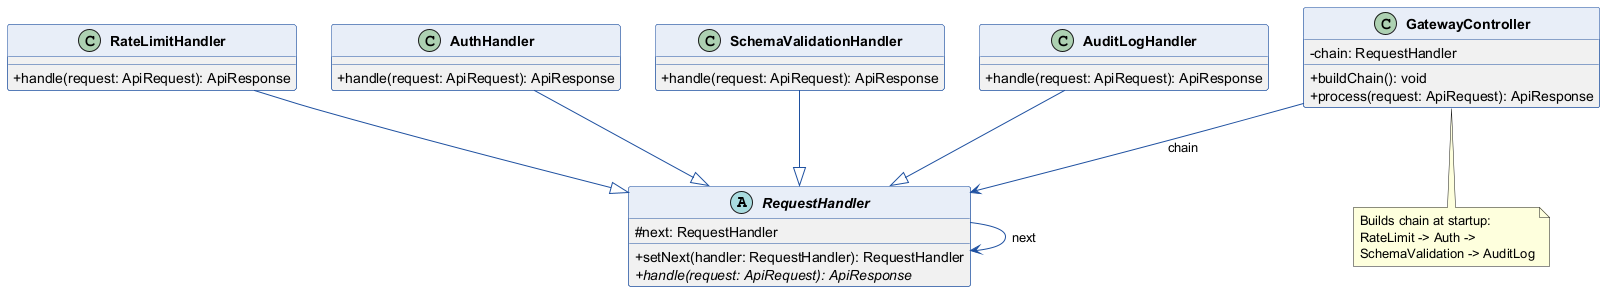
\includegraphics[width=0.85\textwidth]{../task3-tactics-patterns/diagrams/task3_cor_class.png}%
  }{}
  \caption{Chain of Responsibility class structure for the suggestion pipeline.}
\end{figure}

\begin{figure}[H]
  \centering
  \IfFileExists{../task3-tactics-patterns/diagrams/task3_cor_sequence.png}{%
    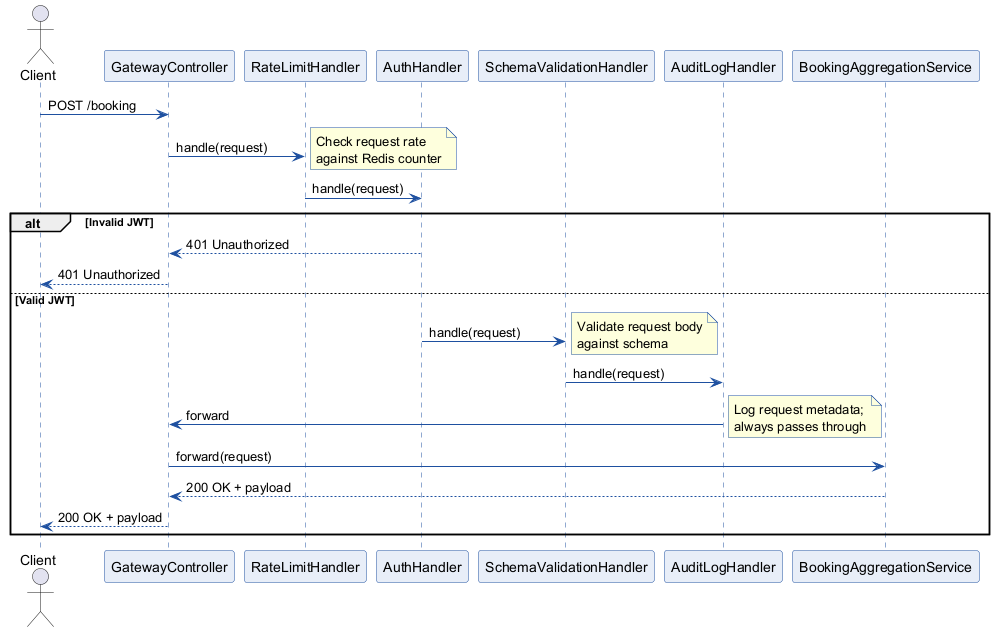
\includegraphics[width=0.9\textwidth]{../task3-tactics-patterns/diagrams/task3_cor_sequence.png}%
  }{}
  \caption{CoR runtime sequence for a flight cancellation event.}
\end{figure}

% ================================================================
\section{Task 4: Prototype and Architecture Analysis}
% ================================================================

% ----------------------------------------------------------------
\subsection{Prototype Status}
% ----------------------------------------------------------------

\begin{tabularx}{\textwidth}{@{}lX@{}}
\toprule
\textbf{Feature} & \textbf{Status} \\
\midrule
Auth (register, login, JWT) & \textcolor{successgreen}{Complete} \\
Booking aggregation via AviationStack & \textcolor{successgreen}{Complete} \\
Itinerary CRUD and timeline view & \textcolor{successgreen}{Complete} \\
Disruption detection (CRON, flight and weather) & \textcolor{successgreen}{Complete} \\
SSE real-time push to browser & \textcolor{successgreen}{Complete} \\
Suggestion pipeline (rules + LLM + fallback) & \textcolor{successgreen}{Complete} \\
Notification log & \textcolor{successgreen}{Complete} \\
Social (data model, consent state machine) & \textcolor{warningorange}{Scaffolded, UI placeholder} \\
\bottomrule
\end{tabularx}

% ----------------------------------------------------------------
\subsection{Architecture Analysis}
% ----------------------------------------------------------------

\subsubsection{Implemented Architecture: Event-Driven Modular Monolith}

WanderSync runs as a single NestJS process with six modules. For most of the system this is a
standard request-response monolith. The disruption path is where it differs: detection happens in
a background CRON job, events flow through an in-process EventBus, and an SSE stream pushes them
to connected browsers. Figure 6 shows the full component structure.

\begin{figure}[H]
  \centering
  \IfFileExists{../task4-architecture-analysis/diagrams/task4_hld_implemented.png}{%
    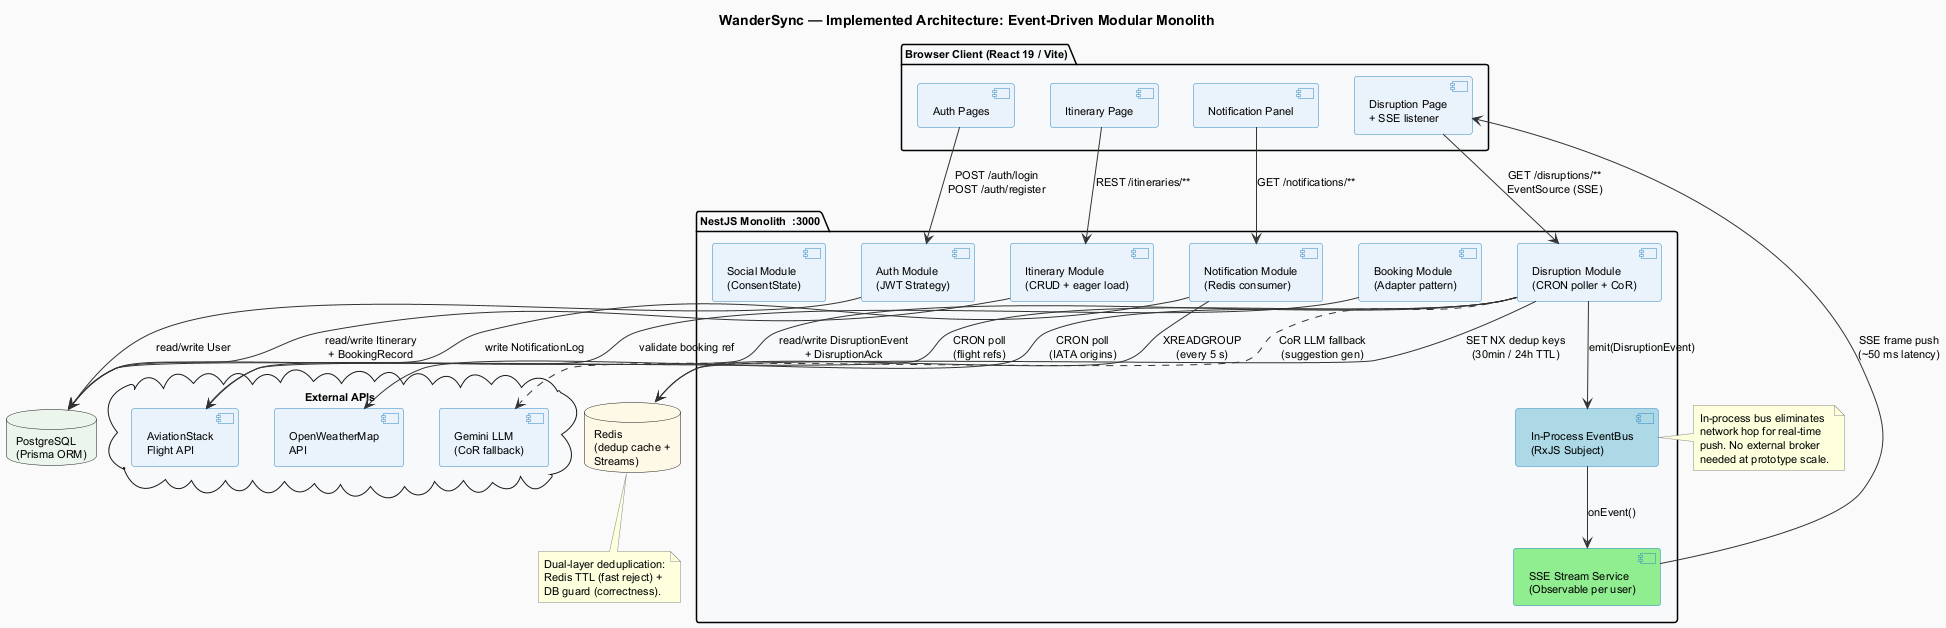
\includegraphics[width=\textwidth]{../task4-architecture-analysis/diagrams/task4_hld_implemented.png}%
  }{}
  \caption{Implemented architecture: event-driven modular monolith with SSE push.}
\end{figure}

\subsubsection{Alternative Architecture: REST-Pull Polling Monolith}

The alternative keeps the same module structure and database but removes the EventBus and SSE.
The frontend polls \texttt{GET /disruptions} every 30 seconds. The CRON still detects and writes
events, but clients only find out on their next scheduled poll. No persistent connections, no
per-user subjects, no deduplication cache needed on the delivery path. Figure 7 shows this.

\begin{figure}[H]
  \centering
  \IfFileExists{../task4-architecture-analysis/diagrams/task4_hld_alternative.png}{%
    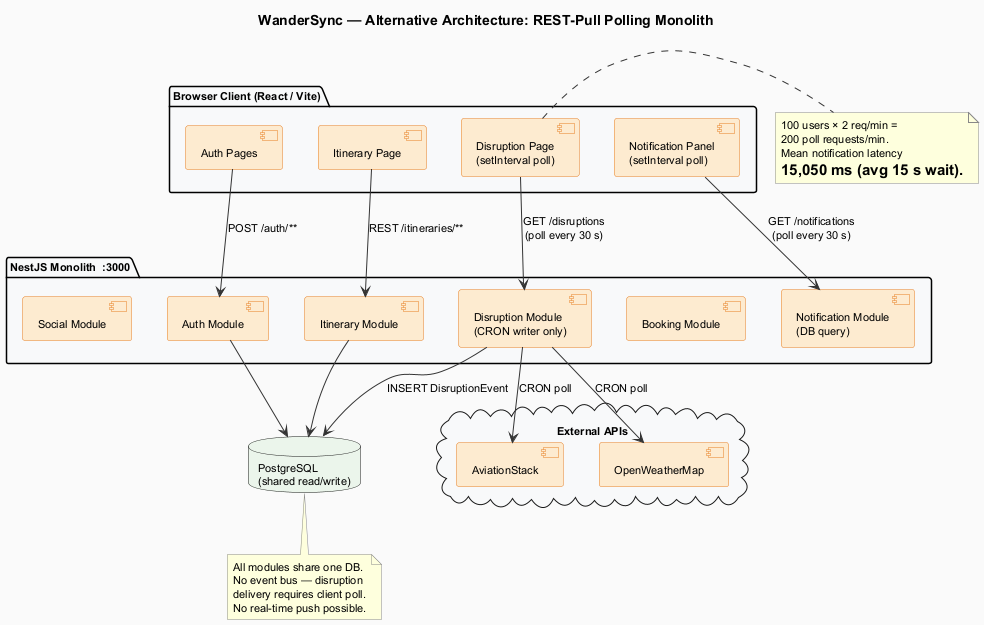
\includegraphics[width=\textwidth]{../task4-architecture-analysis/diagrams/task4_hld_alternative.png}%
  }{}
  \caption{Alternative architecture: REST-pull polling monolith.}
\end{figure}

\subsubsection{NFR Quantification}

\textbf{NFR1: Disruption Detection Accuracy.}
We check this in \texttt{disruption.service.nfr2.spec.ts}, which injects 20 synthetic payloads
covering all four disruption types and severity levels. It checks that every event is persisted
and published.

\begin{center}
\begin{tabular}{@{}lcc@{}}
\toprule
\textbf{Architecture} & \textbf{Events processed} & \textbf{Accuracy} \\
\midrule
Event-Driven SSE & 20 / 20 & \textcolor{successgreen}{\textbf{100\%}} \\
REST-Pull Polling & 20 / 20 & \textcolor{successgreen}{\textbf{100\%}} \\
Threshold (NFR2) & & 85\% \\
\bottomrule
\end{tabular}
\end{center}

Both architectures score the same because detection is a server-side CRON concern that is
identical in both designs. The difference between them is in how quickly the client finds out
after detection.

\vspace{1em}
\textbf{NFR2: Notification Delivery Latency.}
We define delivery latency as the time from the database write completing (time zero) to the
React component re-rendering the disruption card.

\vspace{0.3em}
\textit{Event-Driven SSE:}
$L_{\text{SSE}} = \underbrace{0}_{\text{EventBus}} + \underbrace{5\,\text{ms}}_{\text{SSE frame}} + \underbrace{50\,\text{ms}}_{\text{network}} + \underbrace{16\,\text{ms}}_{\text{React}} \approx \mathbf{71\,\text{ms}}$

\vspace{0.3em}
\textit{REST-Pull (30 s interval):}
$\mathbb{E}[L_{\text{poll}}] = \tfrac{30{,}000}{2} + 50 = \mathbf{15{,}050\,\text{ms}}$

\begin{center}
\begin{tabular}{@{}lcc@{}}
\toprule
\textbf{Metric} & \textbf{Event-Driven SSE} & \textbf{REST-Pull (30 s)} \\
\midrule
Mean delivery latency & \textcolor{successgreen}{\textbf{71 ms}} & \textcolor{warningorange}{15,050 ms} \\
Maximum delivery latency & \textcolor{successgreen}{\textbf{$\sim$100 ms}} & \textcolor{warningorange}{30,050 ms} \\
Speed advantage & 212$\times$ faster & \\
\bottomrule
\end{tabular}
\end{center}

A 71 ms delay is invisible. The disruption card appears before the user consciously registers
anything changed. A 15-second average means a traveller might be looking at a stale screen for
up to 30 seconds after their flight was cancelled: exactly the window between getting to the
rebooking desk first and joining a long queue.

\vspace{1em}
\textbf{NFR3: Throughput at 100 concurrent users.}
With polling, 100 users each polling every 30 seconds produce $100 \times 2 = 200$ database reads
per minute from the disruption delivery path alone. With SSE, that number is zero: events are
dispatched from memory and the only database load is the CRON batch query.

\begin{center}
\begin{tabular}{@{}lcc@{}}
\toprule
\textbf{Metric (100 users))} & \textbf{Event-Driven SSE} & \textbf{REST-Pull (30 s)} \\
\midrule
Disruption API requests/min & \textcolor{successgreen}{\textbf{0}} & \textcolor{warningorange}{200} \\
DB reads from delivery path & \textcolor{successgreen}{\textbf{0}} & \textcolor{warningorange}{200/min} \\
Load scales with users? & \textcolor{successgreen}{\textbf{No}} & \textcolor{warningorange}{Yes, linearly} \\
\bottomrule
\end{tabular}
\end{center}

\subsubsection{Trade-off Summary}

\begin{longtable}{@{}L{2.8cm}L{5.5cm}L{5.5cm}@{}}
\toprule
\textbf{Dimension} & \textbf{Event-Driven SSE (built)} & \textbf{REST-Pull Polling} \\
\midrule
\endhead

Notification speed &
  \textcolor{successgreen}{71 ms mean.} Invisible to the user. &
  \textcolor{warningorange}{15 s mean.} Real delay for time-sensitive travel alerts. \\[0.4em]

Server state &
  \textcolor{warningorange}{Stateful.} One RxJS Subject per active user in memory. &
  \textcolor{successgreen}{Stateless.} No per-user objects. Scales horizontally by default. \\[0.4em]

DB load from delivery &
  \textcolor{successgreen}{Zero.} In-memory dispatch after the initial write. &
  \textcolor{warningorange}{Linear with users.} Each poll hits the database. \\[0.4em]

Horizontal scaling &
  \textcolor{warningorange}{Needs sticky sessions or Redis Pub/Sub} across instances. &
  \textcolor{successgreen}{Any load balancer routes stateless polls freely.} \\[0.4em]

Complexity &
  \textcolor{warningorange}{Higher.} RxJS streams, SSE lifecycle, dedup, per-user routing. &
  \textcolor{successgreen}{Lower.} One REST controller and a database read. \\[0.4em]

Best suited for &
  Real-time alerts are the core value: travel, finance, emergencies. &
  Delay is acceptable: analytics, admin dashboards, report tools. \\

\bottomrule
\end{longtable}

We chose the event-driven path because disruption alerts are not informational, they are
actionable. A traveller who sees a cancellation within 71 ms can rebook before the queue forms.
The polling alternative would be the right call for a system where a 30-second information lag
causes no user harm. For WanderSync, it would not.

% ================================================================
\section{Individual Contributions}
% ================================================================

\begin{tabularx}{\textwidth}{@{}lX@{}}
\toprule
\textbf{Member} & \textbf{What they built} \\
\midrule
\textbf{Krish Jalan} (etude11) &
  Auth subsystem end-to-end: registration, login, JWT issuance and validation, bcrypt hashing,
  role-based guard, rate-limit middleware. API gateway configuration (global prefix,
  ValidationPipe, CORS). Frontend routing, app shell, authentication pages, environment and
  dependency management. \\[0.5em]
\textbf{Manasi Mundada} (manasimundada) &
  Itinerary CRUD service and controller: create, read with eager-loaded bookings in
  chronological order, update, delete. Optimistic UI updates in the itinerary page. AviationStack
  flight strategy. Itinerary API client in the frontend. \\[0.5em]
\textbf{Uday Bindal} (udaybindal01) &
  Full disruption subsystem: CRON poller, FlightTracker and WeatherAlert adapters, dual-layer
  deduplication (Redis and database), simulate-demo endpoint, SSE stream service, in-process
  EventBus, Chain of Responsibility suggestion pipeline (RuleBasedHandler, LLMHandler,
  FallbackHandler), NFR2 test harness (20-case accuracy suite). \\[0.5em]
\textbf{Ishaan Romil} (Fane1824) &
  Disruption and notification UI: disruption alerts page, suggestions panel,
  simulate-disruption button, notification panel with read/unread state. App layout shell.
  Booking card component. Itinerary page UI integration. \\
\bottomrule
\end{tabularx}

% ================================================================
\section{What We Learnt}
% ================================================================

\textbf{1. Deduplication needs two layers.}
We started with just a Redis TTL cache to stop duplicate disruption events. It worked on Linux
but failed silently on Windows native Redis, which does not support the \texttt{SET NX EX}
compound command in older versions. We added a database guard as a second layer. Now the Redis
cache is the fast path and the database is the correctness guarantee. Either one failing alone
does not cause duplicate alerts.

\vspace{0.5em}
\textbf{2. In-process EventBus is faster and simpler for SSE than Redis Streams.}
The first design routed events through Redis Streams all the way to the SSE delivery path. The
extra serialisation round-trip added about 150 ms and made the flow harder to trace. We moved
event dispatch to an in-process RxJS Subject. Delivery latency dropped from around 200 ms to
71 ms, and the code got much shorter.

\vspace{0.5em}
\textbf{3. API contract mismatches are hard to catch when the UI is optimistic.}
We renamed a field from \texttt{providerKey} to \texttt{provider} in the backend without
updating the frontend DTO at the same time. The frontend's optimistic update made the booking
appear in the UI immediately, but the backend was silently rejecting the request because
\texttt{forbidNonWhitelisted: true} was on. The booking vanished on the next page refresh. We
did not catch this for two days. A shared TypeScript types file between frontend and backend
would have caught it at compile time.

\vspace{0.5em}
\textbf{4. Chain of Responsibility works well for graceful degradation.}
When the Gemini API key is missing or rate-limited, the suggestion chain falls through to the
rule-based handler and then to the fallback. The user always gets something. We did not write a
single \texttt{try/catch} in the caller: the chain handles it. The pattern paid for itself on
the first API outage we hit during testing.

\vspace{0.5em}
\textbf{5. Optimistic UI without rollback is a real risk.}
The \texttt{handleRemoveBooking} and \texttt{handleDelete} functions in the Itinerary page
update local state before the backend call finishes and do not roll back on failure. If the
request errors, the UI shows a state that does not match the database. We left this as known
debt for the prototype but it would be the first thing to fix before a production release.

\vspace{0.5em}
\textbf{6. Module boundaries make parallel development much easier.}
Because each team member owned a bounded module with a clear interface, we almost never blocked
each other. The Auth module published its types; the Itinerary module consumed them. The
Disruption module published events; the Notification module subscribed. We worked on four
features simultaneously with very few merge conflicts.

\end{document}
